\clearpage
\subsection{premi/client/utility}
\begin{figure}[H]
\begin{center}
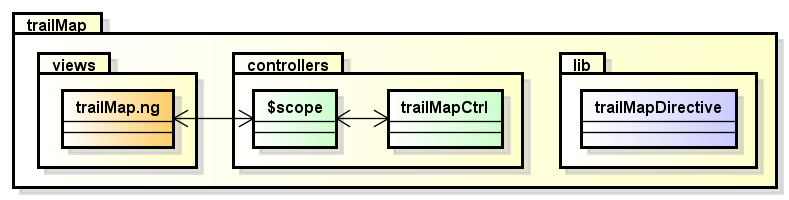
\includegraphics[scale=0.70]{img/diapkg/trailMap.png}
\caption{Diagramma della classe premi/client/trailMap}
\end{center}
\end{figure}

%-------  diagramma di un template %
\subsubsection{premi/client/utility/views/actionDialog.ng}

\begin{description}
%-------  descrizione del template%
\item[Descrizione] \hfill
	template della vista associato alla direttiva \textit{actionDialogDirective} che permette di visualizzare un messaggio all'utente	
\end{description}

%-------  diagramma di un template %
\subsubsection{premi/client/utility/lib/actionDialogDirective}

\begin{description}
%-------  descrizione del template%
\item[Descrizione] \hfill
	direttiva che include la vista \textit{actionDialog.ng} e permette con il tag html$_G$ \textit{action-dialog} di visualizzare un messaggio all'utente che può essere personalizzato includendo codice html tra il tag di apertura e chiusura della direttiva
\end{description}